\label{sec:background}
In diesen Kapitel soll die Problemstellung der mangelhaften Softwaredokumentation analysiert werden. Hierzu muss zunächst der Begriff \enquote{Softwaredokumentation} definiert werden. Anschließend werden einige Statistiken präsentiert, die zeigen, dass eine mangelhafte Softwaredokumentation ein reales Problem für Entwickler ist. Des Weiteren sollen die Folgen von schlecht dokumentierten Code analysiert werden. Zudem wird in diesem Kapitel die Grundlagen von Javadocs erläutert, welches das Tool später als Grundlage für die Analyse der Dokumentation nutzt. Zuletzt werden noch einige Programme vorgestellt, die unter anderem auch die Dokumentation von Software bewerten können. 

\section{Definition der Softwaredokumentation}
Um den Begriff \enquote{Softwaredokumentation} zu definieren, sollte zunächst der Begriff \enquote{Dokumentation} definiert werden. Das IEEE  definiert diesen Begriff als jede textliche oder bildliche Information, welche Aktivitäten, Anforderungen, Abläufe oder Ergebnisse beschreibt, definiert, spezifiziert, berichtet oder zertifiziert \cite[S. 28]{IEEEStandardGlossaryofSoftwareEngineeringTerminology}. Kurz zusammengefasst beschreibt eine Dokumentation also, wie sich eine Komponente aufgebaut ist oder wie sie sich verhält.

Diese abstrakte Definition lässt sich so auf Softwareentwicklung übertragen. In \cite[S. 125]{Softwaredocumentationandstandards} wird Softwaredokumentation als eine Sammlung von technischen Informationen beschrieben, die für Menschen lesbar sind und die die Funktionen, Benutzung oder das Design eines Softwaresystems beschreiben. So beschreibt der Autor in [], dass die Hauptaufgabe beim Programmieren nicht sein sollte, einen Computer zu erklären, was er machen sollte, sondern anderen Menschen zu erklären, was der Computer machen sollte.

Im Kontext dieser Bachelorarbeit sollen allerdings nur bestimmte Arten der Softwaredokumentation betrachtet werden, da eine umfassende Betrachtung innerhalb der vorgegebenen Zeit nicht möglich ist. Die wichtigste Kategorie im Kontext der Bachelorarbeit sind bestimmte Kommentare im Quelltext eines Programms, die zu den sogenannten Inline-Kommentaren gehören. Diese Kommentare werden wie normale Kommentare erkannt und werden daher nicht Bestandteil des kompilierten Programms. Nichtsdestotrotz haben diese spezifischen Kommentare aber eine bestimmte Struktur, die eine leichte Verarbeitung durch Computerprogramme ermöglicht und gleichzeitig trotzdem für Menschen lesbar bleibt. In vielen Fällen werden diese Kommentare einer bestimmten Komponente zugeordnet, wobei dies oft dadurch geschieht, dass der Kommentar direkt vor dieser Komponente steht.

Andere Möglichkeiten zur Dokumentation, die nur hier kurz erwähnt werden sollen, sind UML-Diagramme, Handbücher und  Readme-Dateien.


\section{Statistiken zu Softwarequalität}
Dass in vielen Fällen die Softwaredokumentation vernachlässigt wird, ist durch viele Studien belegt. Eine Umfrage aus dem Jahr 2002 mit 48 Teilnehmern belegt beispielsweise, dass Anforderungs- oder Spezifikationsdokumente nur selten bei Änderungen am Quellcode angepasst werden. Außerdem verwenden viele Entwickler häufig Programme, die nicht für Dokumentationszwecke entwickelt wurden (z. B Microsoft Word etc.) \cite[S. 28-29]{TheRelevanceofSoftwareDocumentationToolsandTechnologies:ASurvey}. Diese Programme sind leicht zu bedienen und sehr flexibel, verwenden jedoch teilweise proprietäre Dateiformate und sind daher nicht unbedingt effizient.

Eine weitere Studie aus dem Jahr 2019 verdeutlicht viele Aspekte aus der vorgenannten Umfrage. Es wurden dabei Daten aus Stack Overflow, GitHub Issues und Pull Requests und Mailing-Listen automatisiert heruntergeladen und dann von den Autoren analysiert, ob und inwieweit mit mangelhafter Softwaredokumentation zu tun haben.  Die Studie liefert klare Indizien dafür, dass die Softwaredokumentation in vielen Fällen nicht komplett, nicht auf dem neuesten Stand oder sogar nicht korrekt ist. Des Weiteren ist die Softwaredokumentation nicht gut nutzbar oder schlecht lesbar, sodass der Vorteil verloren geht\cite[S.1201 -1204]{SoftwareDocumentationIssuesUnveiled}.
\section{Javadoc}
Javadoc \cite{Javadoc} ist ein Tool zur Generierung von Dokumentationen, das sich als de-facto Standard für Dokumentationen in der Programmiersprache Java etabliert hat \cite[S. 249]{JavadocViolationsandTheirEvolutioninOpen-SourceSoftware}.  Javadoc besteht aus speziellen Java-Kommentaren, die an bestimmten Stellen im Quellcode eingefügt werden und daher bei der Kompilation nicht berücksichtigt werden. Ein Javadoc-Block beschreibt immer ein bestimmtes Modul (z. B. eine Klasse, Methode oder Feld).Es beginnt mit der Zeichenkette \enquote{/**}, wobei die ersten beiden Zeichen \enquote{/*} den Beginn eines mehrzeiligen Kommentars in Java einläuten, und endet mit \enquote{*/}. Zunächst sollte am Anfang des Blocks eine generelle Zusammenfassung der Komponente geschrieben werden. Danach können sogenannte Tags, die mit dem \enquote{@}-Zeichen beginnen, benutzt werden. Diese beschreiben wiederum einen bestimmten Teilbereich einer Komponente. Es ist zudem Konvention, dass jede Zeile in einem Javdoc-Block mit einem Asterisk beginnt. Tabelle \ref{tab:table_javadoc_method} beschreibt einige Tags für Java-Methoden:
\begin{table}[h]
    \centering
    \begin{tabular}{m{4cm}|m{4cm}|m{7cm}}
    Tag & zusätzliche Parameter &Beschreibung\\
    \hline
        @param  & Paramatername & Beschreibt einen Methodenparameter\\
        \hline
         @return & & Beschreibt den Rückgabewert der Methode, sofern er existiert \\
         \hline
         @throws &Exception & Beschreibt welche Exceptions diese Methode werfen kann und möglichst unter welchen Umständen dies passiert \\
           \hline
         @deprecrated & & Falls diese Methode veraltet ist und nicht mehr verwendet werden sollte, kann hier eine Alternative beschrieben werden. \\
           \hline
         
           \hline
         
         
         
         
    \end{tabular}
    \caption{Wichtige Javadoc-Tags}
    \label{tab:table_javadoc_method}
\end{table}
Listing \ref{lst:simple_javadoc} zeigt ein Beispiel für eine  \enquote{gelungene} Verwendung von Javadoc. Zunächst wird der Zweck der Methode beschrieben, anschließend wird jeder Parameter erläutert. Dabei sollte in komplexeren Fällen auch erklärt werden, welche Werte gültig für den Parameter sind. Danach folgt eine Beschreibung des Rückgabewertes, welche am besten auch jeden möglichen Fall abdeckt. Mit \enquote{{@code ...}} kann auf einen Parameter referenziert werden. Mit diesen Informationen kann der Programmierer leicht überblicken, wie eine Methode genutzt werden, sodass die Einarbeitungszeit und die Fehleranfälligkeit reduziert werden kann.  
		\begin{figure}
			\lstinputlisting
			[caption={Beispielhafter Javdoc-Block für einfache Methode},
			label={lst:simple_javadoc}
			captionpos=b,language=java, basicstyle=\footnotesize, tabsize=1, showstringspaces=false,  numbers=left]
			{figures/ternary.java}
		\end{figure}

Auf der offiziellen Oracle-Webseite werden weitere empfehlenswerte Tipps für gute Javadoc-Kommentare gegeben, die hier auszugsweise und ohne besondere Reihenfolge wiedergegeben werden\cite{HowtoWriteDocCommentsfortheJavadocTool}:
\begin{itemize}
    \item Nicht in jeden Fall vollständige Sätze verwenden, aber klar formulieren, was die Aufgabe einer Komponente ist
    \item In der dritten und nicht in der zweiten Person schreiben
    \item Nicht repetitiv sein. Ein Kommentar, der im Wesentlichen nur den Namen einer Komponente wiedergibt, hat keinen Mehrwert
    \item  Beschreibungen von Methoden sollten mit einem Verb beginnen
    \item bei einem Verweis auf das aktuelle Objekt sollte das spezifische \textit{this} statt des allgemeineren \textit{the} verwendet werden
    \item Bezeichner sollten in mit \textit{<code></code>} umschlossen werden, um deutlich zu machen, dass dies eine andere Komponente ist
    \item Der Kommentar sollte eventuelle Unterschiede unter verschiedene Plattformen erläutern
    \item Die Dokumentation sollte erläutern, wie sich die Komponente in Randfällen verhält
    
\end{itemize}
Diese Javadoc-Blöcke können dann von dem gleichnamigen Tool in eine HTML-Datei umgewandelt werden und ermöglichen den Entwicklern damit einen komfortablen Überblick über alle Komponenten eines Moduls. Zudem könne Javadoc-Blöcke ebenfalls HTML-Inhalte besitzen, die dann von Javadoc in die HTML-Datei übernommen werden, sodass der Entwickler beispielsweise Tabellen zur übersichtlichen Präsentation  von Informationen verwenden kann. Abbildung \ref{fig:javadoc_example_screenshot} zeigt, wie eine Methode mittels Javadoc in HTML beschrieben wird. 
\begin{figure}[h]
    \centering
    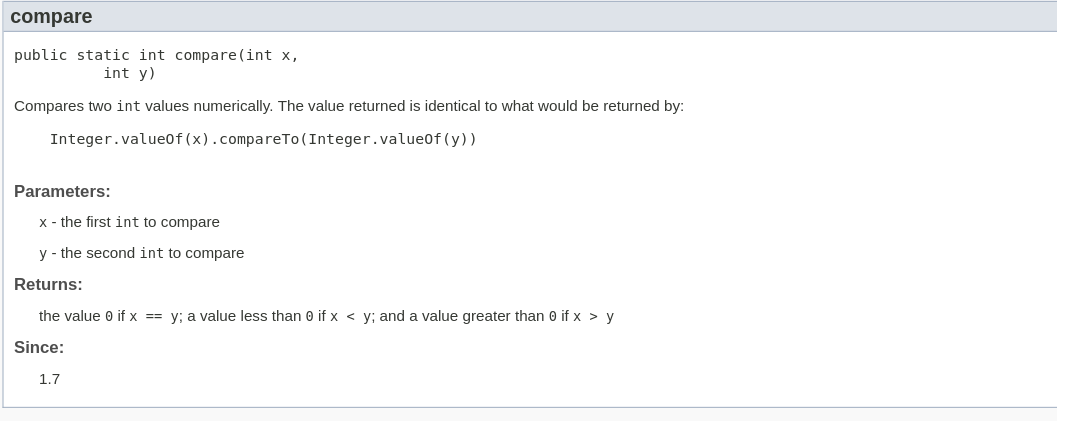
\includegraphics[width=\columnwidth]{figures/javadoc_screenshot.png}
    \caption{Gerenderte HTML-Ausgabe von javadoc}
    \label{fig:javadoc_example_screenshot}
\end{figure}

in Javadoc-Kommentar wird vererbt und muss daher für eine abgeleitete Klasse nicht neu geschrieben oder redundant geklont werden. Dies ist sinnvoll, da abgeleitete Klassen einen Vertrag erfüllen müssen, der bei einer guten Dokumentation auch schon in der Javadoc-Dokumentation beschrieben wird. Auch bei Methoden, die aufgrund einer Schnittstelle implementiert werden müssen, ist eine Neudefinition des Javadoc-Kommentar unnötig. Falls sinnvoll, kann aber dennoch ein eigener Javadoc-Kommentar erstellt werden, der allerdings den Kommentar der Quelle vollständig ersetzt. Mit \textit{@inheritDoc} kann der ursprüngliche Kommentar aber trotzdem eingefügt werden.

Für andere Programmiersprachen gibt es vergleichbare Werkzeuge, die ähnliche Funktionen anbieten und bei denen die Dokumentationen mit einer relativ ähnlichen Syntax erstellt werden. Dazu gehören beispielsweise Doxygen für C++-Programme oder der PHP-Documentor für PHP-Programme. 
\section{Tools zur Bewertung von Javadoc}
Um die Qualität der Softwaredokumentation in Javadoc zu bewerten, gibt es bereits einige Programme. In vielen Fällen handelt es sich dabei um Programme, die nicht auf die Bewertung der Softwaredokumentation beschränkt sind, sondern auch andere Fälle von unsauberem Code erkennen können. Da die Bewertung der Dokumentation nicht der primäre Zweck der Programme ist, sind die verwendeten Metriken recht allgemein und erkennen viele Problemfälle nicht. Nichtsdestotrotz sind diese Programme, dadurch dass sie viele \enquote{Code-Smells} erkennen, sehr gut geeignet, um sich ein gutes Bild über die Qualität des Quellcodes zu verschaffen und den Entwickler zu sauberer Arbeit auch außerhalb von Kommentaren zu ermuntern.

Eines der bekanntesten Programme ist Checkstyle. Mit Checkstyle lässt sich beispielsweise prüfen, ob alle Methoden überhaupt ein Javadoc-Block besitzen, der Javadoc-Block korrekt platziert wurde oder ein Javadoc-Tag wie zum Beispiel \enquote{@deprecated} auch mit einer zusätzlichen Begründung versehen wurde. 

Des Weiteren gibt es das Programm PMD, das ebenfalls einige Metriken für Javadoc mitliefert. Dazu gehört, ob jede öffentliche Methode dokumentiert wurde oder die Kommentare generell zu lang sind. Interessanterweise gibt es auch die Möglichkeit, bestimmte Wörter, die als anstößig empfunden werden, aus Kommentaren und Dokumentationen auszuschließen, damit Kommentare neutral bleiben. 

Das oben erwähnte Javadoc-Tool bietet ebenfalls die Möglichkeit, beim Generieren der HTML-Datei die Qualität des Javadocs zu prüfen. Dabei werden vor allem fehlende Tags für Parameter etc. bemängelt. Zudem erkennt Javadoc auch Tabellen mit fehlender Überschrift und andere Designmängel, die in der HTML-Seite später auffallen. Auch fehlerhaftes HTML kann erkannt werden.

\section{Theoretische Arbeiten im Bereich der Bewertung von Softwaredokumentation}

Neben den praktischen Tools, die den Softwareentwickler bei der Bewertung der Softwaredokumentation unterstützen, wurden auch einige wissenschaftliche Arbeiten veröffentlicht, die sich mit Metriken über Softwaredokumentation auseinandersetzen. 

Die wichtigste Arbeit, die eine Grundlage dieser Bachelorarbeit ist, ist der \enquote{JavaDocMiner} \cite[S. 68-79]{AutomaticQualityAssessmentofSourceCodeComments:TheJavadocMiner}. In dieser Arbeit wird ein Programm beschrieben, welches mittels einfachen \ac{NLP}-Heuristiken eine Einschätzung der Softwaredokumentation beschrieben. Dabei beschränkt sich der JavaDocMiner nur auf Java-Programme, während das hier zu entwickelnde Tool  auch mit anderen Programmiersprachen zurechtkommen soll. 